


Definir o que é um bom algoritmo de segmentação


avaliação
todos precisam de um gold text

	1 - Concatenação
	2 - Juízes concordam ou não 
	3 - Mediador na reunião
	4 - Não avaliar o segmentador e sim o resultado da aplicação final.
	5 - Consultar o autor do texto
	
	

De acordo com \cite{fulano} há duas principais dificuldades na avaliação de segmentadores automáticos. A primeira é conseguir um referência confiável de texto segmentado, ou seja, uma segmentação ideal, já que juízes humanos costumam não concordar entre si, sobre onde os limites estão. A segunda é que tipos diferentes de erros devem ter pesos diferentes de acordo com a aplicação. Há casos onde certa imprecisão é tolerável e outras como a segmentação de notícias, onde a precisão é mais importante.

Para contornar essas dificuldades, algumas abordagens podem ser utilizadas. Algumas autores preferem detectar a segmentação em textos formados pela concatenação de documentos distintos, para que não haja diferenças subjetivas \cite{Reynar 1994; Choi 2000; e própiro autor do "A Critique and Impro.}. Há ainda outros que não avaliam o algoritmo diretamente, mas seu impacto na aplicação final\cite{Manning 1998; Kan,
Klavans, and McKeown 1998}. 
Outras abordagens apenas atribuiem um segmento cada quebra de parágrafo \cite{Two Step ... Meeting Minutes}


% Dificuldade: Coesão léxica não tão bem definida
O vocabulário das reuniões, ainda que em tópicos diferentes, compartilham certo vocabulário pertencente ao ambiente onde as se deram as reuniões. Isso é um fator que diminui a o princípio da coesão léxica entre os segmentos.


\subsection{Medidas de Avaliação}


	As medidas de avaliação tradicionalmente utilizadas em \textit{information retrieval} como precisão e revocação trazem alguns problemas na avalização de segmentadores automáticos.  
Conforme o algoritmo aponta mais segmentos no texto, tende a melhorar a revocação e ao mesmo tempo, reduzir a precisão, um problema que pode ser contornado usando F1 que faz uma combinação da duas levando em conta seus pesos, o que por outro lado é mais difícil de interpretar. 
Essas medidas falham ao não serem sensíveis a \textit{near misses}, ou seja, quando um limite não coincide exatamente com o esperado, mas fica próximo~\cite{Kern2009167}.

A Figura~\ref{fig:exemplosegmentacaozoom} mostra um exemplo com duas segmentações hipotéticas e uma referência. Em ambos os casos não há nenhum verdadeiro positivo, o que implica em zero para os valores de precisão, acurácia, e revocação, embora a segunda hipótese possa ser considerada superior à primeira se levado em conta a proximidade dos limites.



  \begin{figure}[!h]

	\centering
	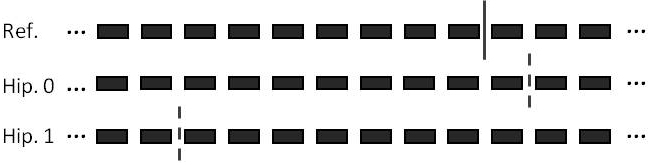
\includegraphics[width=0.47\textwidth]{windiffzoom.jpg}
	\caption{Exmplos de segmentação}
	\label{fig:exemplosegmentacaozoom}

  \end{figure}



\subsubsection{P$_k$}
A fim de resolver o problema de \textit{near misses}, Beeferman \textit{at al.}~\cite{Beeferman1999} apresentam uma nova medida chama P$_k$ que atribui valores parciais a \textit{near misses}. Esse método move uma janela de tamanho $k$ e a cada posição e verifica se o inicio e o final da janela estão dentro do segmento esperado e penaliza o algoritmo em caso de discrepância.
% divide o número de discrepâncias pela quantidade de limites analizados 


\subsubsection{WindowDiff}

Pevzner~\cite{Pevzner200219} aponta problemas na avaliação mais tradicional Pk~\cite{Beeferman1999}. Eles apontam que esse métrica penaliza demasiadamente os falsos negativos em relação aos falsos positivos, desconsidera no o tamanho e a quantidade de segmentos, entre outros apontamentos.

Como solução, propõe duas alterações principais. Dobra a penalidade para os falsos positivos a fim de diminuir o problema da subestimação dessa medida e

ao mover a janela pelo texto e penaliza o algoritmo sempre que o número de limites proposto pelo algoritmo não coincidir com o número de limites esperados para aquela janela de texto. 


%\textit{near misses}, quando um limite entre tópicos não casa exatamente com esperado mas fica próximo a ele.


  \begin{figure}[!h]

	\centering
	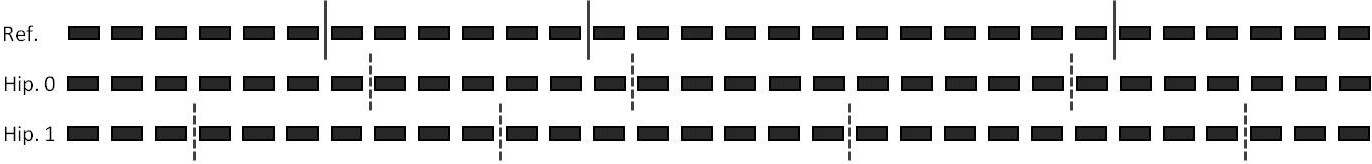
\includegraphics[width=0.47\textwidth]{windiff.jpg}
	\caption{Exemplo de construção de uma matriz de rank}
	\label{fig:exemplosegmentacao}

  \end{figure}

